% CVPR 2023 Paper Template
% based on the CVPR template provided by Ming-Ming Cheng (https://github.com/MCG-NKU/CVPR_Template)
% modified and extended by Stefan Roth (stefan.roth@NOSPAMtu-darmstadt.de)
\documentclass[10pt,twocolumn,letterpaper]{article}

%%%%%%%%% PAPER TYPE  - PLEASE UPDATE FOR FINAL VERSION
% \usepackage[review]{cvpr}      % To produce the REVIEW version
\usepackage{cvpr}              % To produce the CAMERA-READY version
%\usepackage[pagenumbers]{cvpr} % To force page numbers, e.g. for an arXiv version


\usepackage{CJKutf8} % For chinese output

% Include other packages here, before hyperref.
\usepackage{graphicx}
\usepackage{amsmath}
\usepackage{amssymb}
\usepackage{booktabs}
\usepackage{xcolor}
\graphicspath{ {./images/} }

% It is strongly recommended to use hyperref, especially for the review version.
% hyperref with option pagebackref eases the reviewers' job.
% Please disable hyperref *only* if you encounter grave issues, e.g. with the
% file validation for the camera-ready version.
%
% If you comment hyperref and then uncomment it, you should delete
% ReviewTempalte.aux before re-running LaTeX.
% (Or just hit 'q' on the first LaTeX run, let it finish, and you
%  should be clear).
\usepackage[pagebackref,breaklinks,colorlinks]{hyperref}


% Support for easy cross-referencing
\usepackage[capitalize]{cleveref}
\crefname{section}{Sec.}{Secs.}
\Crefname{section}{Section}{Sections}
\Crefname{table}{Table}{Tables}
\crefname{table}{Tab.}{Tabs.}


%%%%%%%%% PAPER ID  - PLEASE UPDATE
\def\cvprPaperID{*****} % *** Enter the CVPR Paper ID here
\def\confName{CVPR}
\def\confYear{2023}


\begin{document}
\begin{CJK*}{UTF8}{bsmi}

%%%%%%%%% TITLE - PLEASE UPDATE
\title{Google - Isolated Sign Language Recognition}

\author{王浩 \\
國立成功大學 資訊工程學系\\
F74082141\\
{\tt\small Howard.H.Wang.23@gmail.com}
% For a paper whose authors are all at the same institution,
% omit the following lines up until the closing ``}''.
% Additional authors and addresses can be added with ``\and'',
% just like the second author.
% To save space, use either the email address or home page, not both
\and
杜孟聰\\
國立成功大學 資訊工程學系\\
F74082028\\
{\tt\small F74082028@gs.ncku.edu.tw}
}
\maketitle

%%%%%%%%% ABSTRACT
\begin{abstract}
   This paper aims to classify isolated American Sign Language (ASL) signs using a deep learning model. 
   To achieve this, we trained the model on labeled landmark data extracted via the MediaPipe Holistic Solution. 
   Our approach leverages the accuracy and reliability of this technology to enhance the robustness of the model and improve its performance. 
   By accurately classifying ASL signs, our method has the potential to support individuals with hearing impairments and 
   enable better communication between hearing and non-hearing populations.
\end{abstract}

%%%%%%%%% BODY TEXT
\section{Introduction}
\label{sec:intro}
Deaf children born to hearing parents are at risk of Language Deprivation Syndrome if they don't have access to a fully developed language early in life. 
However, learning American Sign Language (ASL) can be time-consuming and resource-intensive for parents. 
Automatic sign language recognition technology can help overcome this barrier by recognizing and translating signs into text or speech.

In this paper, we propose a novel approach to isolated sign language recognition using computer vision techniques and machine learning algorithms. 
Our approach improves accuracy, robustness, and speed, as demonstrated on a publicly available dataset.
%-------------------------------------------------------------------------
\subsection{American Sign Language}

American Sign Language (ASL) is a language used primarily by members of the Deaf community in North America. 
It is not a visual representation of English, but has its own unique grammar, syntax, and vocabulary. 
ASL is a visual-gestural language, meaning that it uses facial expressions, body language, and hand movements to convey meaning.

\subsection{Isolated Sign Language Recognition}

ISLR stands for Isolated Sign Language Recognition, which is the task of recognizing individual signs or tokens called glosses from a given segment of signing video clip.
It is the process of recognizing sign language gestures performed by a person in isolation, without considering the context or the surrounding gestures. 
We will train a machine learning model that can accurately recognize isolated sign language signs and classify them into the correct sign category.

%------------------------------------------------------------------------
\section{Explorative Data Analysis}
\label{sec:formatting}

%-------------------------------------------------------------------------
\subsection{Raw Data Format}
MediaPipe Holistic Solution~\cite{https://doi.org/10.48550/arxiv.1906.08172} is a powerful, easy-to-use software tool that can detect and track multiple human body parts and gestures in real-time video streams. 
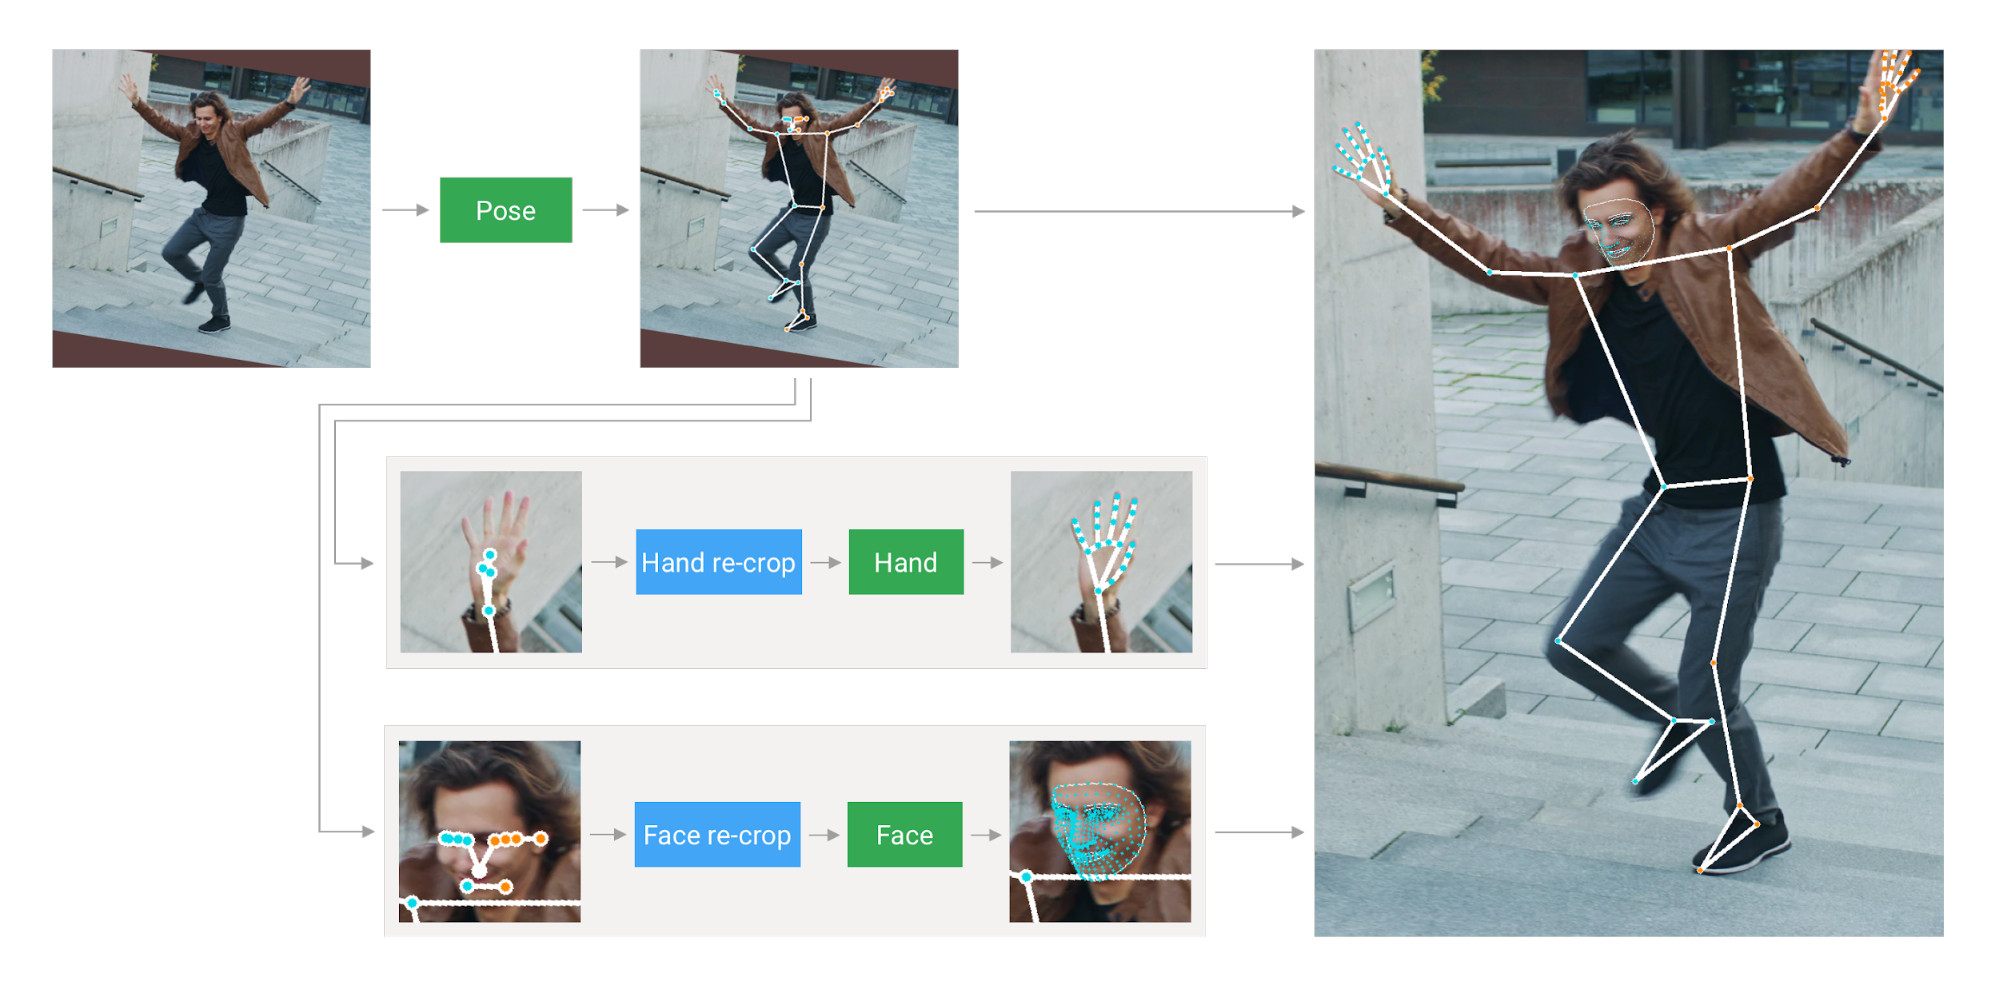
\includegraphics[width=80mm]{holistic_pipeline_example}
The way that MediaPipe Holistic Solution records facial expressions, body language, and hand movements is by using landmarks.

Landmarks or keypoints are like dots that are placed on important areas of an object or a person's body. 
These dots help a computer to understand where these important areas are and how they are moving.

%------------------------------------------------------------------------
\subsection{Data Selection}
{\color{blue} 
The data utilized in this study was obtained from Mediapipe’s Holistic solution and contains landmarks from three categories: Face, Pose (body), and Hand.
In accordance with established linguistic norms, movements below the chest are generally not utilized in sign language for conveying linguistic meanings, therefore, we will exclude landmarks from the hips down and retain only the relevant landmarks for Pose landmarks. Although facial expressions are not an integral part of signing, they can still play a role in identifying words that require the signer to point to parts of the face. Furthermore, facial expressions can provide subtle cues to differentiate between similar signs. Thus, we will utilize landmarks for the major features of the face: eyes, eyebrows, nose, and lips, and trim out the rest. Given the crucial role of hands in sign language, all Hand landmarks will be included in our training data. In summary, our model will be trained using landmarks from the arms, hands, and major facial features to recognize isolated signs.
}

%------------------------------------------------------------------------
\subsection{Data Imputation}
{\color{blue} 

As described in the competition’s guidelines, not all frames’ Hand data are complete. We have identified two categories with respect to the nature of the missed Hand data:
The first category is where the hand rests idle below the waist. In sign language, there are signs that require only one hand to convey meaning. In such cases, the signer usually rests the other hand at their side, and the missed landmarks on this hand can be disregarded.
The second category involves hands that are raised around the chest or face. A hand in these positions usually indicate that it is actively being used to sign. In such cases, certain techniques need to be employed to deal with these lost data. In cases where hand data is lost in some frames but not others, interpolation can be employed to fill the gaps. The reliability of this method may depend on the number of subtle movements between the frames and the size of the gaps. Alternatively, if the loss of hand data is too substantial (e.g., if no hand data exists across the entire clip), discarding the clip altogether may be the best option. Another viable approach to imputing missed data is to use statistical methods such as averaging measures from other data with the same label. However, complications may arise when the number of frames differs across clips, even when they correspond to the same sign.

}

%------------------------------------------------------------------------

\section{Input Data Format}
\label{sec:formatting}

%-------------------------------------------------------------------------

\subsection{Hierarchical Encoding}
{\color{blue} 
Rather than plotting all landmarks on a shared “global” coordinate system, we will map landmarks onto a hierarchy of local coordinate systems based on the articulation of joints and muscles. We propose that organizing landmark coordinates in a hierarchical structure may help reduce the impact of variations in different realizations of the same sign.
Hypothesis 1. Organizing landmark coordinates in a hierarchical structure in a gesture recognition task can help reduce the impact of variations in different realizations of the same sign.
The reasoning to Hypothesis 1. is that, for most signs, it does not matter whether the hands are slightly below the chest or above it nor does it matter whether it is slightly outside of shoulder width or slightly within, i.e. slight variations in the relative position does not typically result in significant semantic differences. Such variations may be observed across differnt signers with differnt body structures and even in the same signer across different instances and, with one global coordinate system, are reflected systematically on all landmark coordinates of the hands. If we instead encode the hand landmarks in the wrists coordinate system, that variation will be eliminated in the hands and only reflected in the wrists and elbows. Since the number of landmarks impacted by this variation significantly decreases in the hierarchical scheme, we assert that this will in general make the model more robust to variations that are not semantically significant.
}
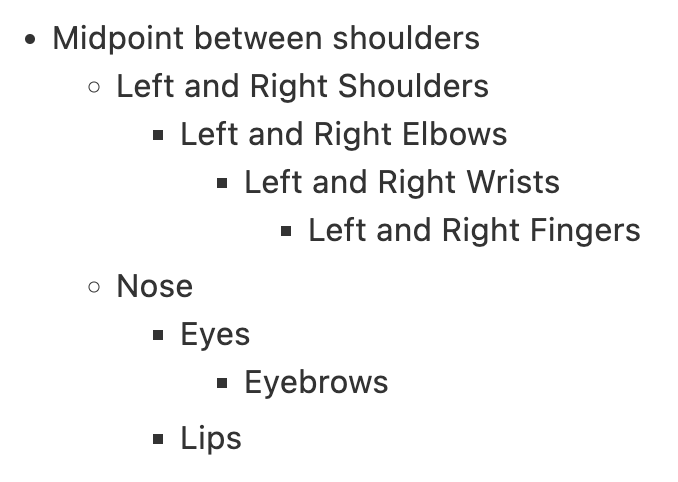
\includegraphics[width=80mm]{hierarchical_scheme}

%------------------------------------------------------------------------

\subsection{Orientation-Focused Encoding}
{\color{blue} 
On top of mapping landmarks onto a hierarchy of coordinate systems, we aim to investigate the impact of an extra encoding scheme on the performance of the model. Specifically, we will explore the effect of encoding only the orientation of landmarks with respect to their origin (i.e., parent) on the final results. To achieve this, we will scale all landmarks down to a uniform size.
On one hand, this approach may help eliminate slight variations in landmark coordinates that arise from individual differences in body structure, such as differences in bone length. On the other hand, since only the x and y coordinates are used in this specific implementation, rotations that do not result in a change in orientation on the xy plane may not be reliably captured. In contrast, if the norm or length of the landmark vectors is also encoded, at least some information about the degree of rotation could be partially captured. For example, the shorter the forearm appears, the more it has rotated towards the observer.
}

%------------------------------------------------------------------------
\subsection{Temporal Normalization by Down-/Upsampling}
{\color{blue} 
Accounting for the different signing speeds among individuals is an important consideration in training a robust sign language recognition model. In practice, signers can vary greatly in their signing speed, and this can result in variations in the rate at which landmarks move from frame to frame. To ensure that our model is not overly sensitive to such differences, we will downsample or upsample the clips to achieve a uniform number of frames. By doing so, we can eliminate any potential errors introduced by variations in the speed at which landmarks move.
}
%------------------------------------------------------------------------

\subsection{Landmark Mirroring}
{\color{blue} 
In sign language, signers commonly rely on a dominant hand to perform the majority of signs, with the specific hand varying among individuals.~\cite{Sign} When signing words that require only one hand, signers typically have the freedom to choose which hand to use. For words that require both hands and involve asymmetric movements, instructions usually designate separate sets of movements for the dominant hand and for the non-dominant hand; it is ultimately up to the signer to decide which hand is dominant.

Thus, for most sign language gestures, flipping the gesture horizontally does not alter its meaning. We have thoroughly examined the dataset and identified no labels such as “left” or “right” for which the choice of dominant hand may affect the meaning. We have thus eliminated concerns for the impact of hand selection in this specific dataset; with that in mind, in our implementation, we will augment the dataset by creating a mirrored version of each clip, enabling the model to learn to recognize the gesture regardless of which hand is designated as dominant.
}
%=========here i am ~~~
%------------------------------------------------------------------------

\section{Model}
{\color{blue}
The Transformer architecture has demonstrated efficacy in sequence-based tasks for dynamic gesture recognition~\cite{TR}. It is important to note that our task differs from the task described in~\cite{TR}, as our input data is comprised of landmark coordinates rather than bitmap images. Specifically, the authors in~\cite{TR} utilize a Convolutional Neural Network (CNN) architecture, ResNet-18, to convert bitmap images into embeddings before feeding them into the Transformer. Despite this difference, we find the Transformer architecture to be a suitable model for our task given its success in a similar domain. Our proposed implementation will use the Transformer with sequences of landmark coordinates as input, and the model will output probabilities for each label.

Our proposed model will consist of a Transformer encoder, followed by a multi-layer perceptron (MLP) decoder. The encoder will be responsible for encoding the input sequence of landmark coordinates into a fixed-length representation, which will then be passed to the decoder to produce the final output probabilities for each label. The MLP decoder will consist of two fully connected layers with ReLU activation functions and a final softmax layer to produce the output probabilities.

To improve the model’s ability to capture temporal dependencies between landmarks, we will also experiment with the use of a Recurrent Neural Network (RNN) architecture as an alternative to the Transformer encoder. In particular, we will explore the use of a Long Short-Term Memory (LSTM) network, which has been shown to be effective in capturing long-term dependencies in sequential data.
}
%------------------------------------------------------------------------
\section{Learning Relative Positions}
In the realm of sign language recognition, the ability to discern relative positions between the hands and other parts of the body is of paramount importance. This becomes particularly evident in situations where the signer points to specific body parts. Moreover, the relative positions between different landmarks of the hands can also significantly influence the recognition process, especially in signs that necessitate the signer to tap one fingertip to another. These relative positions can provide crucial information that aids the recognizer in accurately interpreting the signs.
In this exploration, we ask ourselves the question of whether a model can independently learn to identify relevant relative positions, given the raw landmark points. The aim is to ascertain whether it is possible to eliminate the need to supply the model with programmatically calculated and selected relative positions between pairs of landmark points, without compromising the accuracy of recognition.

A significant trade-off is evident in this scenario. The number of relative positions among 
$n$
 points is calculated as 
$\frac{nx(n-1)}{2}$
, which has a complexity of 
$O(n^2)$
. This could considerably increase the computational complexity during inference and backpropagation. Conversely, if explicit relative positions are entirely omitted in the inputs, the model will be compelled to learn them independently, if at all. This might prolong the time required for convergence.

To better understand this trade-off, we propose two distinct approaches for training the sign language recognizer.
%------------------------------------------------------------------------
\subsection{Entrusting the Model with Extraction of Useful Relative Positions}
In the first approach, we identify a set of landmarks, which include keypoints from the eyes, nose, lips, and the hand. We refer to this set as an ‘anchor group’. These keypoints are then fed into a frame-wise multi-level perceptron (MLP) layer. The underlying hypothesis here is that the MLP can learn to extract useful relative positions between these keypoints in each frame and subsequently utilize them for recognition.
%------------------------------------------------------------------------
\subsection{Explicit Computation of Relative Positions}
The second approach takes a more direct route. Rather than entrusting the model with the task of extracting useful relative positions, we compute these positions explicitly in a feature expansion layer. In this scenario, the model’s primary task is to identify which relative positions are useful, without the added burden of having to extract them.
%------------------------------------------------------------------------
\section{Early Integration vs Late Integration}
Inspired by the dichotomy between early and late fusion strategies in multi-modal learning as delineated in ~\cite{Boulahia2021}, our study delves into a similar contrast between early integration and late integration of different “feature groups” in the context of sign language recognition.
%------------------------------------------------------------------------
\subsection{Feature Grouping: Distinguishing Between Learning Shapes and Spatial Relations}
In our approach, we categorize sets of landmark points into distinct groups, each of which serves a unique purpose. These groups can be broadly classified into three types: “local groups”, “anchor groups”, and the “difference group”.

“Local groups” refer to groups that represent specific body parts, such as the hand, lips, etc. The primary objective of these groups is to enable the model to learn the “shape” of the corresponding body parts.

“Anchor groups”, which are already introduced in the last section, are groups of keypoints from different body parts, designed to facilitate the learning of relative positions.

Lastly, the “difference group” is a selected collection of computed differences (relative positions) between landmark points.

The role of “anchor groups” or the “difference group” is to allow the model to learn the “spatial relations” between different body parts or landmarks.

In our model, irrespective of the scheme we choose to adopt, all features of the same group are initially fed into a Multi-Layer Perceptron (MLP) to obtain a group-level representation. Integration, in this context, refers to the amalgamation of different group-level representations into a single, unified embedding. This integration could occur either before or after the transformer layer, i.e., early if before and late if after. Furthermore, this integration could involve any number of groups and could be between groups of the same type or of different types. In our exploration, we specifically focus on one particular variety of integration at two different stages; namely, we investigate how integrating “shape” and “spatial relations” information at different stages of the model affects performance.

%------------------------------------------------------------------------
\subsection{Early Integration: A Unified Approach}
In the early integration approach, at the frame level, information from all different feature groups is consolidated into a single vector before the transformer attempts to learn how this unified representation evolves over time by comparing the frames. This scheme necessitates only one unifying transformer, and the final MLP classifier solely takes the output from this single transformer as input.
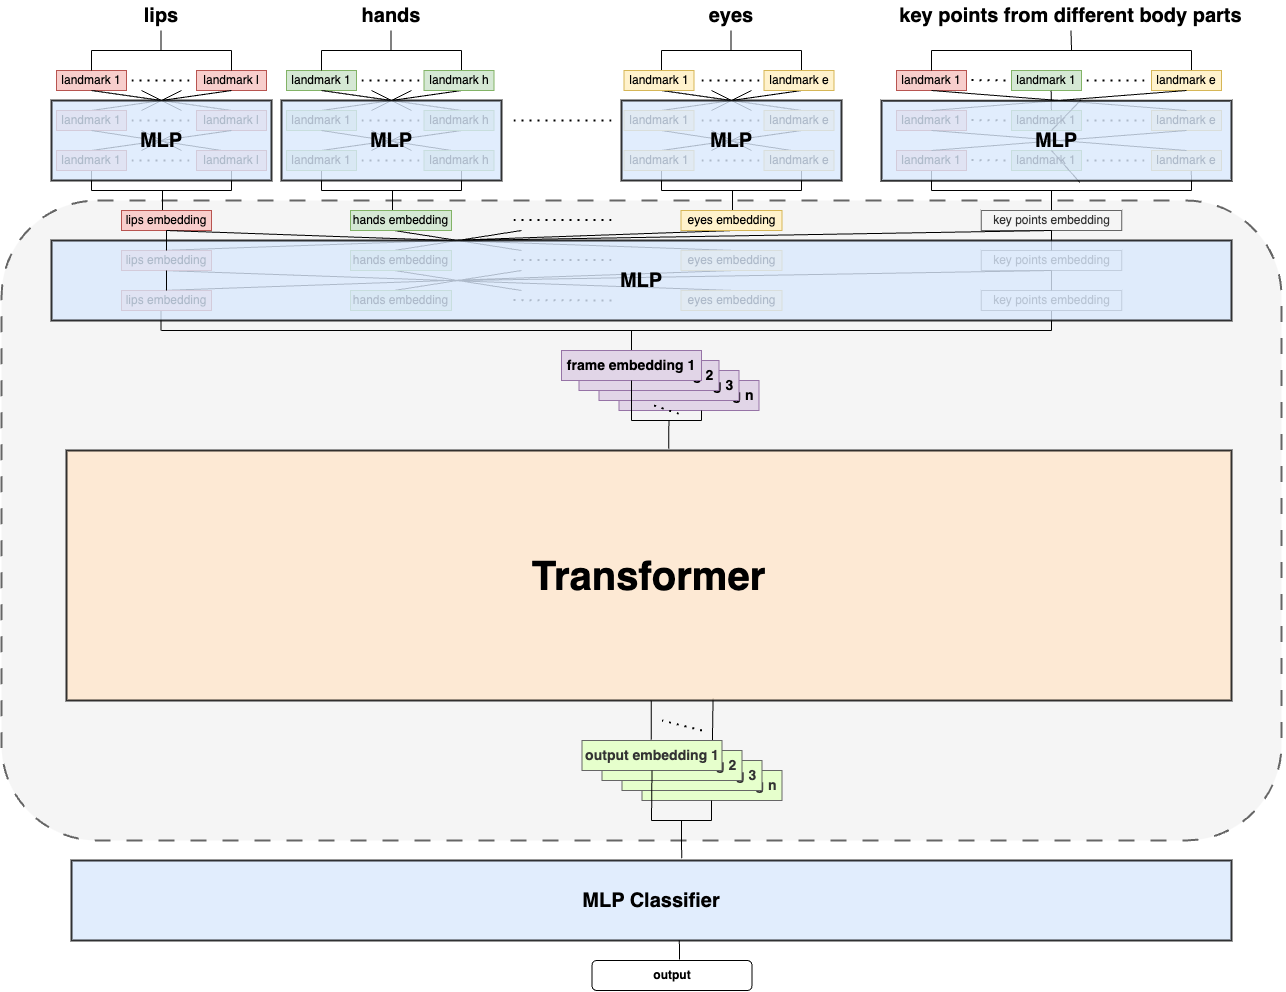
\includegraphics[width=80mm]{early_integration.drawio}
%------------------------------------------------------------------------
\subsection{Late Integration: A Multi-Transformer Approach}
Contrarily, in the late integration approach, information from different group types is represented as separate embeddings at the frame level. This necessitates multiple transformers, one for the “shape” embeddings and another for the “spatial relations” embeddings, to process how these two types of information change along the temporal dimension. Finally, the output embeddings from each transformer are combined before being fed into the final MLP classifier.
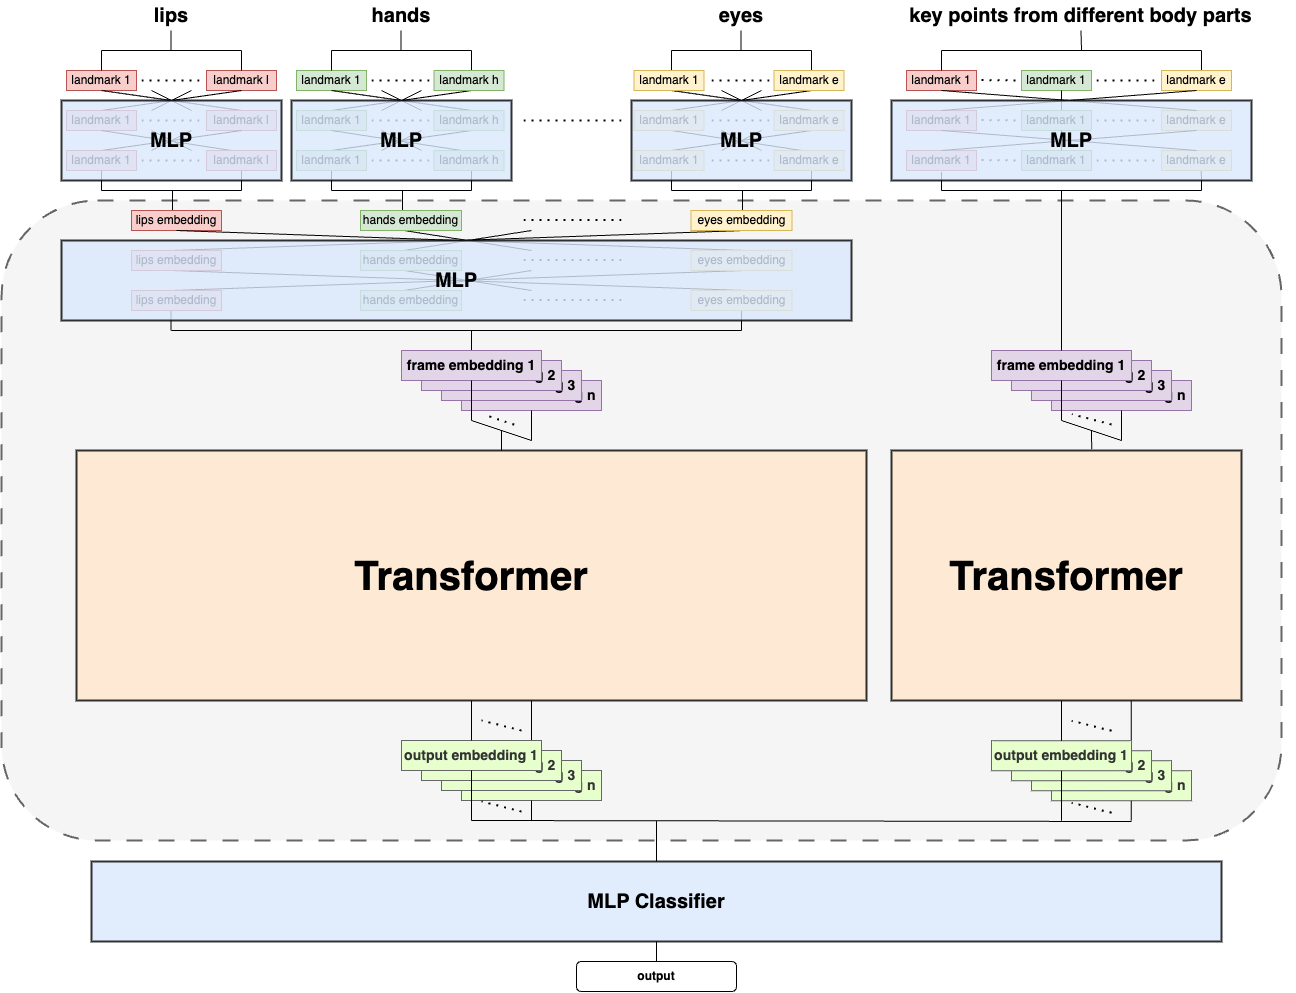
\includegraphics[width=80mm]{late_integration.drawio}
%------------------------------------------------------------------------
\section{Result}
Our model, which utilizes the input data of every video frame's landmarks captured by the MediaPipe Holistic Solution, 
gets the accuracy $0.73$ of isolated sign language recognition.
The parameters of our model are Early Integration with Anchor Group and final layer of model for dimension is $512$. Futhermore, the best score on Kaggle is $0.89$.
We have done that the model will achieve high recognition rates for individual signs, 
thus aiding in the communication and language acquisition process of individuals who are deaf or hard of hearing. 
We believe that our research will contribute to the development of more sophisticated and efficient sign language recognition technology, 
making communication more accessible for the Deaf community.
%------------------------------------------------------------------------

%%%%%%%% REFERENCES
{\small
\bibliographystyle{ieee_fullname}
\bibliography{egbib}
}

\end{CJK*}
\end{document}

